%You can leave alone everything before Line 84.
\documentclass{article}
\usepackage{graphicx}
\usepackage{url,amsfonts, amsmath, amssymb, amsthm, hyperref, subcaption}
% Page layout
\setlength{\textheight}{8.75in}
\setlength{\columnsep}{2.0pc}
\setlength{\textwidth}{6.5in}
\setlength{\topmargin}{0in}
\setlength{\headheight}{0.0in}
\setlength{\headsep}{0.0in}
\setlength{\oddsidemargin}{0in}
\setlength{\evensidemargin}{0in}
\setlength{\parindent}{0pc}
\newcommand{\shortbar}{\begin{center}\rule{5ex}{0.1pt}\end{center}}
%\renewcommand{\baselinestretch}{1.1}
% Macros for course info
\newcommand{\courseNumber}{MATH 510}
\newcommand{\courseTitle}{Intro to Neuro Computation}
\newcommand{\semester}{Fall 2017}
% Theorem-like structures are numbered within SECTION units
\theoremstyle{plain}
\newtheorem{theorem}{Theorem}[section]
\newtheorem{lemma}[theorem]{Lemma}
\newtheorem{corollary}[theorem]{Corollary}
\newtheorem{proposition}[theorem]{Proposition}
\newtheorem{statement}[theorem]{Statement}
\newtheorem{conjecture}[theorem]{Conjecture}
\newtheorem{fact}{Fact}
%definition style
\theoremstyle{definition}
\newtheorem{definition}[theorem]{Definition}
\newtheorem{example}{Example}
%\newtheorem{problem}{Problem}
\newtheorem{exercise}{Exercise}
\newtheorem{algorithm}{Algorithm}
%remark style
\theoremstyle{remark}
\newtheorem{remark}[theorem]{Remark}
\newtheorem{reduction}[theorem]{Reduction}
%\newtheorem{question}[theorem]{Question}
\newtheorem{question}{Question}
%\newtheorem{claim}[theorem]{Claim}
%
% Proof-making commands and environments
\newcommand{\beginproof}{\medskip\noindent{\bf Proof.~}}
\newcommand{\beginproofof}[1]{\medskip\noindent{\bf Proof of #1.~}}
\newcommand{\finishproof}{\hspace{0.2ex}\rule{1ex}{1ex}}
\newenvironment{problem}[1]{\medskip\noindent{\bf Problem #1.~}}{\shortbar}
\newenvironment{solution}[1]{\medskip\noindent{\bf Solution #1.~}}{\shortbar}
%====header======
\newcommand{\solutions}[2]{
%\renewcommand{\thesolution}{{\large #2}.\arabic{problem}}
\vspace{-2ex}
\begin{center}
{\small  \courseNumber, \courseTitle
\hfill {\large \bf {#1} }\\
\semester, University of Oregon \hfill
{\em Andrew Hampton}}\\
\vspace{-1ex}
\hrulefill\\
\vspace{4ex}
\end{center}
}

\setcounter{section}{-1}

\begin{document}
%%%%%%%%%%%%%%%%%%%%%%%%%%%%%%%%%%%%%%%%%%%%%%%%%
\solutions{Project Paper}{December 5, 2017}

\textbf{Biologically plausible learning in recurrent neural networks reproduces neural dynamics observed during cognitive tasks} \\
\textit{Thomas Miconi} \\
\textit{eLife 6 (2017): e20899} \\
\textit{https://www.ncbi.nlm.nih.gov/pmc/articles/PMC5398889} \\

\textbf{Summary}: In this paper, the author presents a novel algorithm for training a recurrent neural network. The algorithm seeks to more accurately represent biological systems than those typically used in machine learning applications. Artificial neural networks have the unrealistic advantage (from a biological perspective) of receiving constant, real-time supervised rewards. By contrast, the author asserts that a biologically plausible network must learn from temporally sparse, discrete rewards. \\

I will only summarize the author's learning rule and the results of my implementation of one particular task. However, in the paper, the author offers a more dramatic claim: that algorithms of the sort presented here offer a model consistent with the learning observed in animal behavior. \\

\textbf{Learning Rule}: The algorithm is based on a recurrent neural network given by the differential equation:

$$
\tau \frac{dx_i}{dt} = -x_i(t) + \sum^N_{j=1}J_{ij}r_j(t) + \sum^M_{k=1}B_{ik}u_k(t).
$$

Here, $\mathbf{x}$ represents the excitation of the neurons and $\mathbf{r}$ the responses. $J$ is an adjacency matrix giving the weights of the internal network, while $B$ represents the weights associated with the external inputs $\mathbf{u}$. \\

The response function used in all of the experiments is:

$$
\mathbf{r}(t) = \tanh(\mathbf{x}(t)).
$$

The particular values of the constants can be found in the paper or the author's \href{https://www.github.com/ThomasMiconi/BiologicallyPlausibleLearningRNN}{code} [1]. Most noteworthy, perhaps, is the initialization of the weight matrix $J$. The entries are initially taken from a normal distribution with mean zero and standard deviation $\frac{g}{\sqrt{N}}$, where $N$ is the number of neurons in the network and $g$ is a constant governing the \textit{chaotic} behavior of the network. The value of $g$ used in these experiments is $1.5$, which allows the network to exhibit chaotic behavior. \\

At every time step of a trial the weight change accumulates in what the author calls a \textit{potential} weight change, given by:

$$
e_{ij}(t) = e_{ij}(t-1) + S(r_j(t-1) \cdot (x_i(t)-\overline{x}_i)).
$$

Here, S is a monotonic, supralinear function (quoting the author: \textit{the plasticity mechanism is dominated by large increments, and tends to suppress smaller ones}) and $\overline{\mathbf{x}}$ is a short-term running average of $\mathbf{x}$. \\

The actual weight update is given by either

$$
\Delta J = \eta e (R - \overline{R})
$$

or

$$
\Delta J = \eta e (R - \overline{R}) \overline{R}.
$$

In these equations, $\eta$ represents the learning rate, $R$ the trial reward, and $\overline{R}$ a running average of the rewards for a given trial type. See the variations on the task below for a more detailed discussion of the implementation of this $\overline{R}$. \\

The first version above appears in the paper while the latter is used in the author's code. Below, we show the results of solving a given task with both versions. \\

\textbf{Delayed XOR Task}: The author presents several tasks, the simplest of which is a basic classification task. Two binary stimuli, whose values are referred to as \textit{A} and \textit{B}, are presented sequentially, and a designated output neuron is trained to emit the value $1$ if the stimulus sequence is \textit{AA} or \textit{BB} and to emit $-1$ in the other two cases. \\

The trial reward (i.e., penalty) is calculated by taking the mean absolute deviation from the expected output over the last $200$ timesteps (where each timestep simulates one millisecond). \\

I replicated the results of this task and performed a few experiments with variations on the parameters [2]. In Figure 1, the results of four variations are presented: \\

\begin{enumerate}
    \item The same task as described in the paper. A table of the reward running average is kept with a separate running average for each of the four trial types. \\

    \item A modified version of the learning rule (the second learning rule given above). Note that the convergence is much more stable in this case. \\

    \item In this version, only two running averages of the reward are kept: one for each of the output cases. We don't observe any learning in this case. \\

    \item Finally, a version which uses a discretized version of the reward: no penalty if the output is on average close to the desired output over the final $200$ timesteps, otherwise a unit penalty. The discrete reward was ineffective. \\
\end{enumerate}

In Figure 2, we see the response of the output neuron over time, taken from the second experimental case described above. The sequence of stimuli after training was \textit{AB}, and we observe the correct behavior. \\

Finally, Figures 3 and 4 show the results of a modification to this task. Keeping a table of running averages of the rewards is somewhat artificial. Instead, we can train four neurons to output the characteristic function of the trial type. Then, we can update all of the running averages each trial, weighted by the respective output neurons. \\

For this alternate formulation of the task, the error was computed by determining which of the four output neurons on average responded closest to the value $1$ over the last $200$ timesteps, then taking the mean absolute deviation of that neuron from $1$. We see that this was model is also successful in learning the task. \\

\begin{figure}
\begin{subfigure}{.5\textwidth}
  \centering
  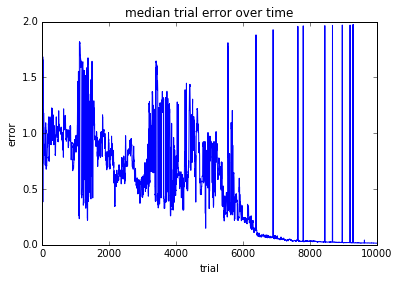
\includegraphics[width=.8\linewidth]{10k_no_rbar}
  \caption{$\Delta J = \eta e (R - \overline{R})$}
  \label{fig:sfig1}
\end{subfigure}%
\begin{subfigure}{.5\textwidth}
  \centering
  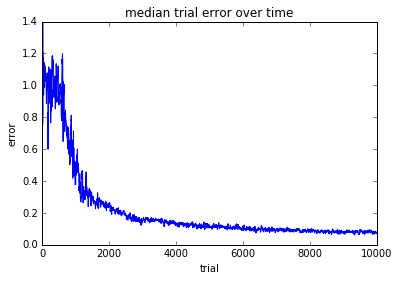
\includegraphics[width=.8\linewidth]{10k_normal}
  \caption{$\Delta J = \eta e (R - \overline{R}) \overline{R}$}
  \label{fig:sfig2}
\end{subfigure}
\begin{subfigure}{.5\textwidth}
  \centering
  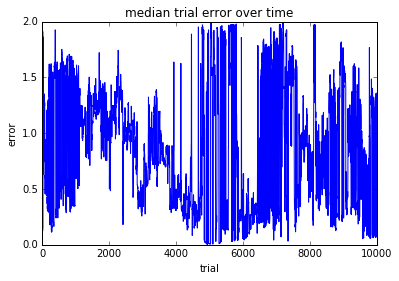
\includegraphics[width=.8\linewidth]{10k_two_bins}
  \caption{Binned learning rule}
  \label{fig:sfig1}
\end{subfigure}%
\begin{subfigure}{.5\textwidth}
  \centering
  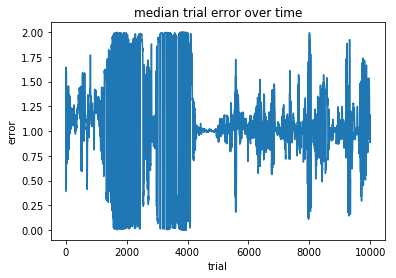
\includegraphics[width=.8\linewidth]{10k_discrete}
  \caption{Discrete learning rule}
  \label{fig:sfig2}
\end{subfigure}
\caption{Error, taken as a rolling median over twenty trials.}
\label{fig:fig}
\end{figure}

\begin{figure}
\begin{subfigure}{.5\textwidth}
  \centering
  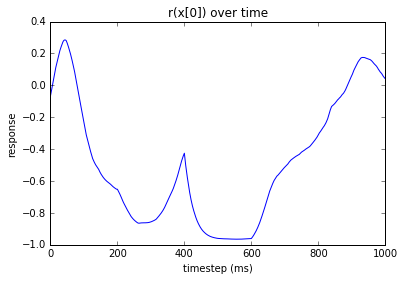
\includegraphics[width=.8\linewidth]{before}
  \caption{Before training}
  \label{fig:sfig1}
\end{subfigure}%
\begin{subfigure}{.5\textwidth}
  \centering
  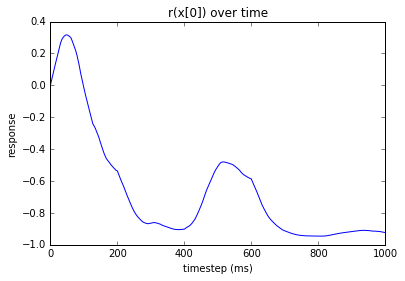
\includegraphics[width=.8\linewidth]{after}
  \caption{After training}
  \label{fig:sfig2}
\end{subfigure}
\caption{Output neuron before and after training during the task of Figure 1b. Observe that, after training, the network has learned to distinguish trial type \textit{AB}.}
\label{fig:fig}
\end{figure}

\begin{figure}
\centering
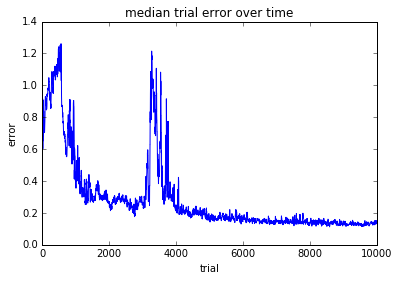
\includegraphics[width=.8\linewidth]{error4}
\caption{Error in alternate formulation of the task, where the characteristic function of the trial type is learned.}
\label{fig:fig}
\end{figure}

\begin{figure}
\begin{subfigure}{.5\textwidth}
  \centering
  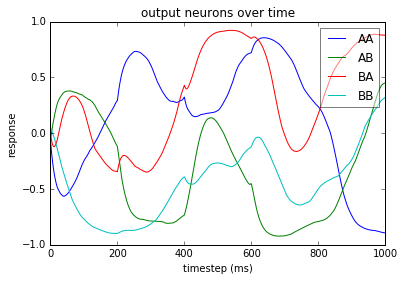
\includegraphics[width=.8\linewidth]{before4}
  \caption{Before training}
  \label{fig:sfig1}
\end{subfigure}%
\begin{subfigure}{.5\textwidth}
  \centering
  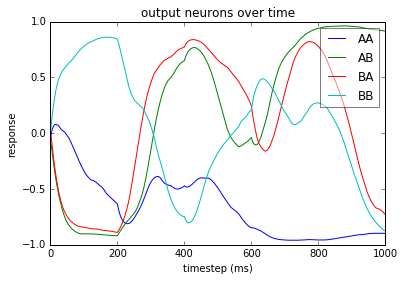
\includegraphics[width=.8\linewidth]{after4}
  \caption{After training}
  \label{fig:sfig2}
\end{subfigure}
\caption{Output neurons before and after training during the task of Figure 3. Observe that, after training, the network has learned to distinguish trial type \textit{AB}.}
\label{fig:fig}
\end{figure}


\textbf{Links}: \\

[1] https://www.github.com/ThomasMiconi/BiologicallyPlausibleLearningRNN

[2] https://www.github.com/awhampton/math510

\end{document}
